\documentclass{article}
\usepackage[utf8]{inputenc}
\usepackage{hyperref}
\usepackage[letterpaper, portrait, margin=1in]{geometry}
\usepackage{enumitem}
\usepackage{amsmath}
\usepackage{booktabs}
\usepackage{graphicx}

\usepackage{hyperref}
\hypersetup{
colorlinks=true,
    linkcolor=black,
    filecolor=black,      
    urlcolor=blue,
    citecolor=black,
}
\usepackage{natbib}

\usepackage{titlesec}
\title{Homework 2}
\author{rbulkunde3 Bulkunde}
\date{January 2023}

\begin{document}

\maketitle

\section{Introduction}
\section{Sample mean table}
 See table \ref{tab:my_label}.

\subsection{Python version}

\begin{table}[ht]
    \centering
    \begin{tabular}{lllr}
\toprule
{} & \multicolumn{2}{l}{Mean} &         Diff \\
{} &    (s.d.) &    (s.d.) &    (p value) \\
\midrule
Electricity (kWh) &   1181.33 &   1086.75 &    -3.403304 \\
                  &  (454.31) &  (423.96) &     0.000692 \\
Home (sqft)       &   1633.05 &   1657.55 &     0.565839 \\
                  &  (682.90) &  (686.27) &     0.571630 \\
Temperature       &     79.89 &     79.89 &     0.016128 \\
                  &    (2.16) &    (1.97) &     0.987135 \\
Observations      &       501 &       499 &  1000.000000 \\
\bottomrule
\end{tabular}

    \caption{Standard deviation are in paranthesis}
    \label{tab:my_label}
\end{table}

\subsection{Stata version}

\begin{table}[ht]
    \centering
    {
\def\sym#1{\ifmmode^{#1}\else\(^{#1}\)\fi}
\begin{tabular}{l*{3}{cccc}}
\hline\hline
                    &\multicolumn{2}{c}{(1)}  &\multicolumn{2}{c}{(2)}  &\multicolumn{2}{c}{(3)}           \\
                    &\multicolumn{2}{c}{}     &\multicolumn{2}{c}{}     &\multicolumn{2}{c}{}              \\
                    &        mean&          sd&        mean&          sd&           b         &           t\\
\hline
electricity         &    1181.329&     454.308&    1086.745&     423.960&      94.584\sym{***}&     (3.404)\\
sqft                &    1633.052&     682.904&    1657.551&     686.271&     -24.499         &    (-0.566)\\
temp                &      79.891&       2.163&      79.893&       1.968&      -0.002         &    (-0.016)\\
\hline
Observations        &         501&            &         499&            &        1000         &            \\
\hline\hline
\end{tabular}
}

    \caption{Summary statistics produced using Stata}
    \label{tab:statasummary}
\end{table}

\section{STATA Regression}
\begin{table}[ht]
    \centering
    \begin{tabular}{lc} \hline
 & (1) \\
VARIABLES & Ordinary least squares \\ \hline
 &  \\
sqft & 0.62** \\
 & (0.01) \\
retrofit & -109.67** \\
 & (7.94) \\
temp & 3.26 \\
 & (1.93) \\
Constant & -83.60 \\
 & (154.69) \\
 &  \\
Observations & 1,000 \\
 R-squared & 0.92 \\ \hline
\multicolumn{2}{c}{ Robust standard errors in parentheses} \\
\multicolumn{2}{c}{ ** p$<$0.01, * p$<$0.05} \\
\end{tabular}

    \caption{Regression produced using Stata}
    \label{tab:Regression}
\end{table}

\section{Graphs}

\subsection{Python version: Kernel Density Plot}

\begin{figure}[ht]
    \centering
    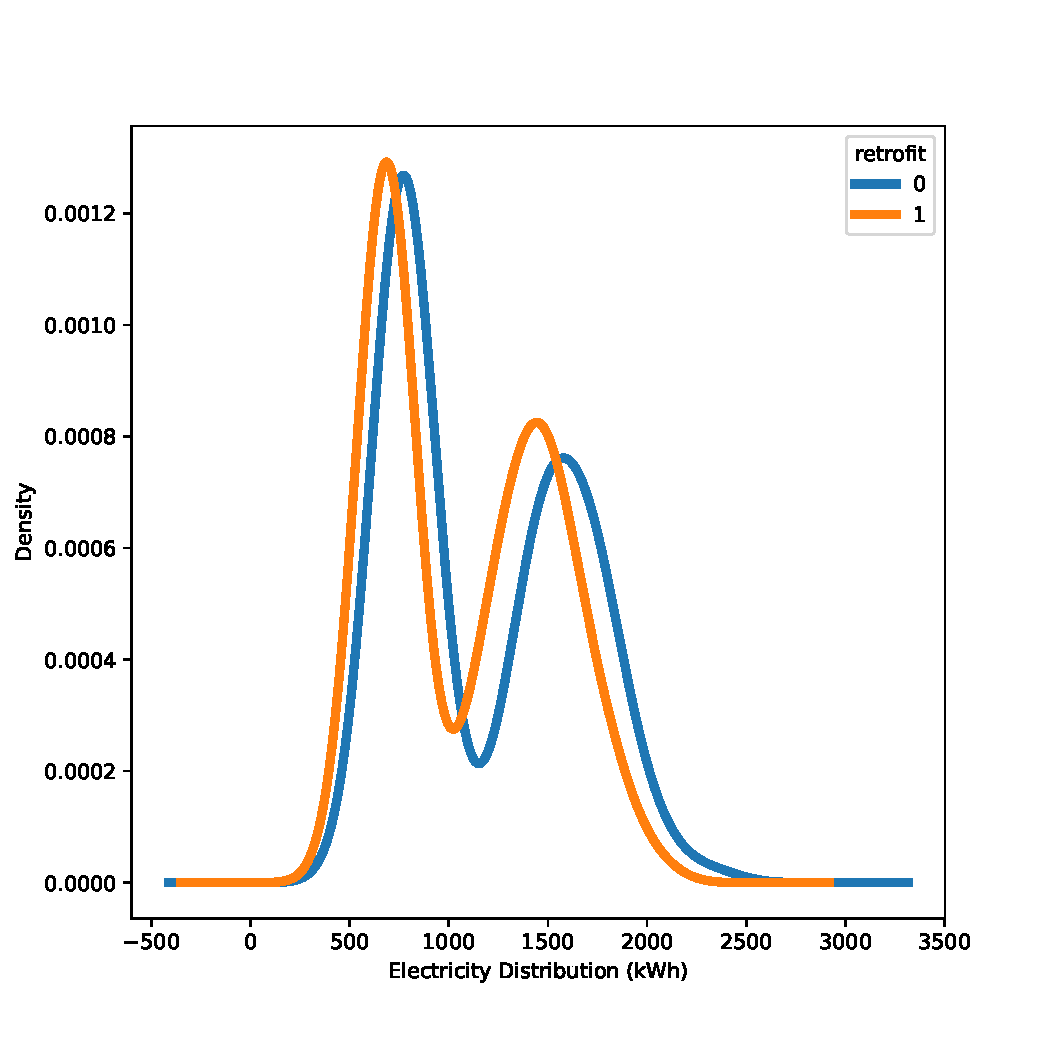
\includegraphics[scale = 0.7]{python_kwh_hist.pdf}
    \caption{Sample kernel density plot of the outcome variable.}
    \label{fig:samplehist}
\end{figure}

\subsection{Stata version: two-way scatterplot}

\begin{figure}[ht]
    \centering
    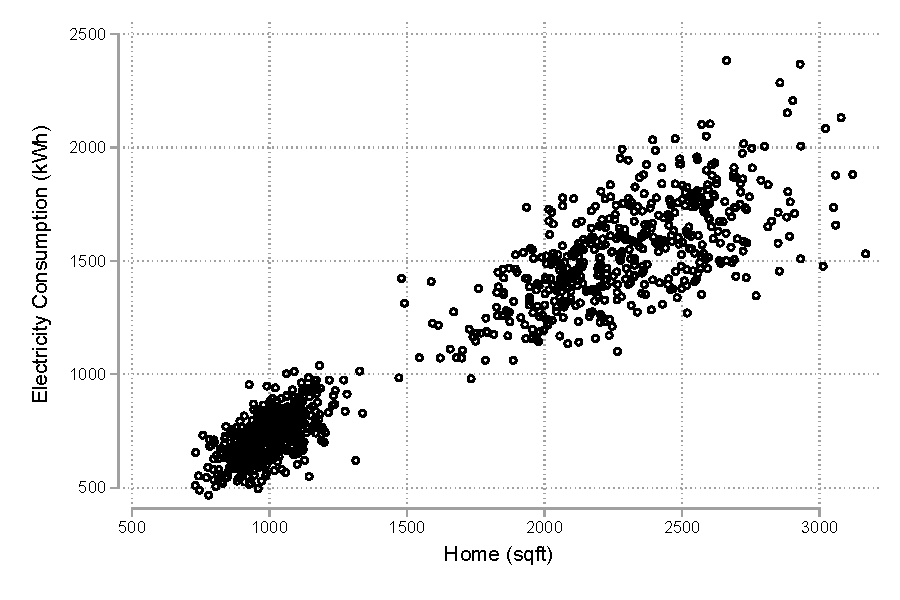
\includegraphics{Stata_twowayscatter.pdf}
    \caption{two-way scatterplot}
    \label{fig:statahist}
\end{figure}

\end{document}
